\section{Datenbankdesign}
Um die Erweiterung der Datenbank für den Feasibility Check zu erklären, wird zunächst auf die grundlegende Struktur der REALIS-Datenbank eingegangen. In Abbildung \ref{fig:realis-datenbankdesign} ist ein Ausschnitt der wichtigsten Tabellen und deren Beziehungen dargestellt, einschließlich der vorgenommenen Erweiterungen, die durch orangefarbenden Rechtecke gekennzeichnet sind. Die nachfolgenden Erläuterungen nennen jeweils den zugehörigen Tabellennamen aus der Abbildung in Klammern.

\subsection{REALIS-Datenbank}

Wie bereits in Kapitel \ref{Subsec:project-lifecycle} beschrieben, besteht ein \textbf{REALIS-Projekt} (\texttt{relproject}), in dem neue Produkte qualifiziert werden, aus mehreren \textbf{Tests} (\texttt{test}). Jeder Test besitzt einen eindeutigen \textbf{State} (\texttt{ctlg\_state\_type}), der zu Beginn auf ''NEW'' gesetzt wird und nach Abschluss den Status ''ARCHIVE'' erhält (vgl. Abbildung \ref{fig:realis-project-lifecycle}, rechte Spalte). Zudem wird jeder Test einer Kategorie bzw. einem \textbf{Test-Typ} (\texttt{ctlg\_test\-\_sub\_type}) zugeordnet.

Ein Test besteht aus mehreren aufeinanderfolgenden \textbf{Operationen} (\texttt{operation}), die nacheinander im \gls{RPT}-Labor abgearbeitet werden. Die Tabellen, die eng mit der Operation verknüpft sind, sind in Abbildung \ref{fig:realis-datenbankdesign} im grün umrandeten Bereich dargestellt. Jede Operation kann dabei einen oder mehrere \textbf{Parameter} (\texttt{op\_data}) enthalten, die beispielsweise die Umgebungsbedingungen definieren. Die konkreten Werte dieser Parameter sind in dem Eintrag \texttt{OPD\_PLAN} hinterlegt. Jeder Parameter ist zudem einer \textbf{Kategorie} (\texttt{ctlg\_op\_\-data\_type}) zugeordnet.  


\begin{figure}[!htbp]
    \centering
    \makebox[\textwidth]{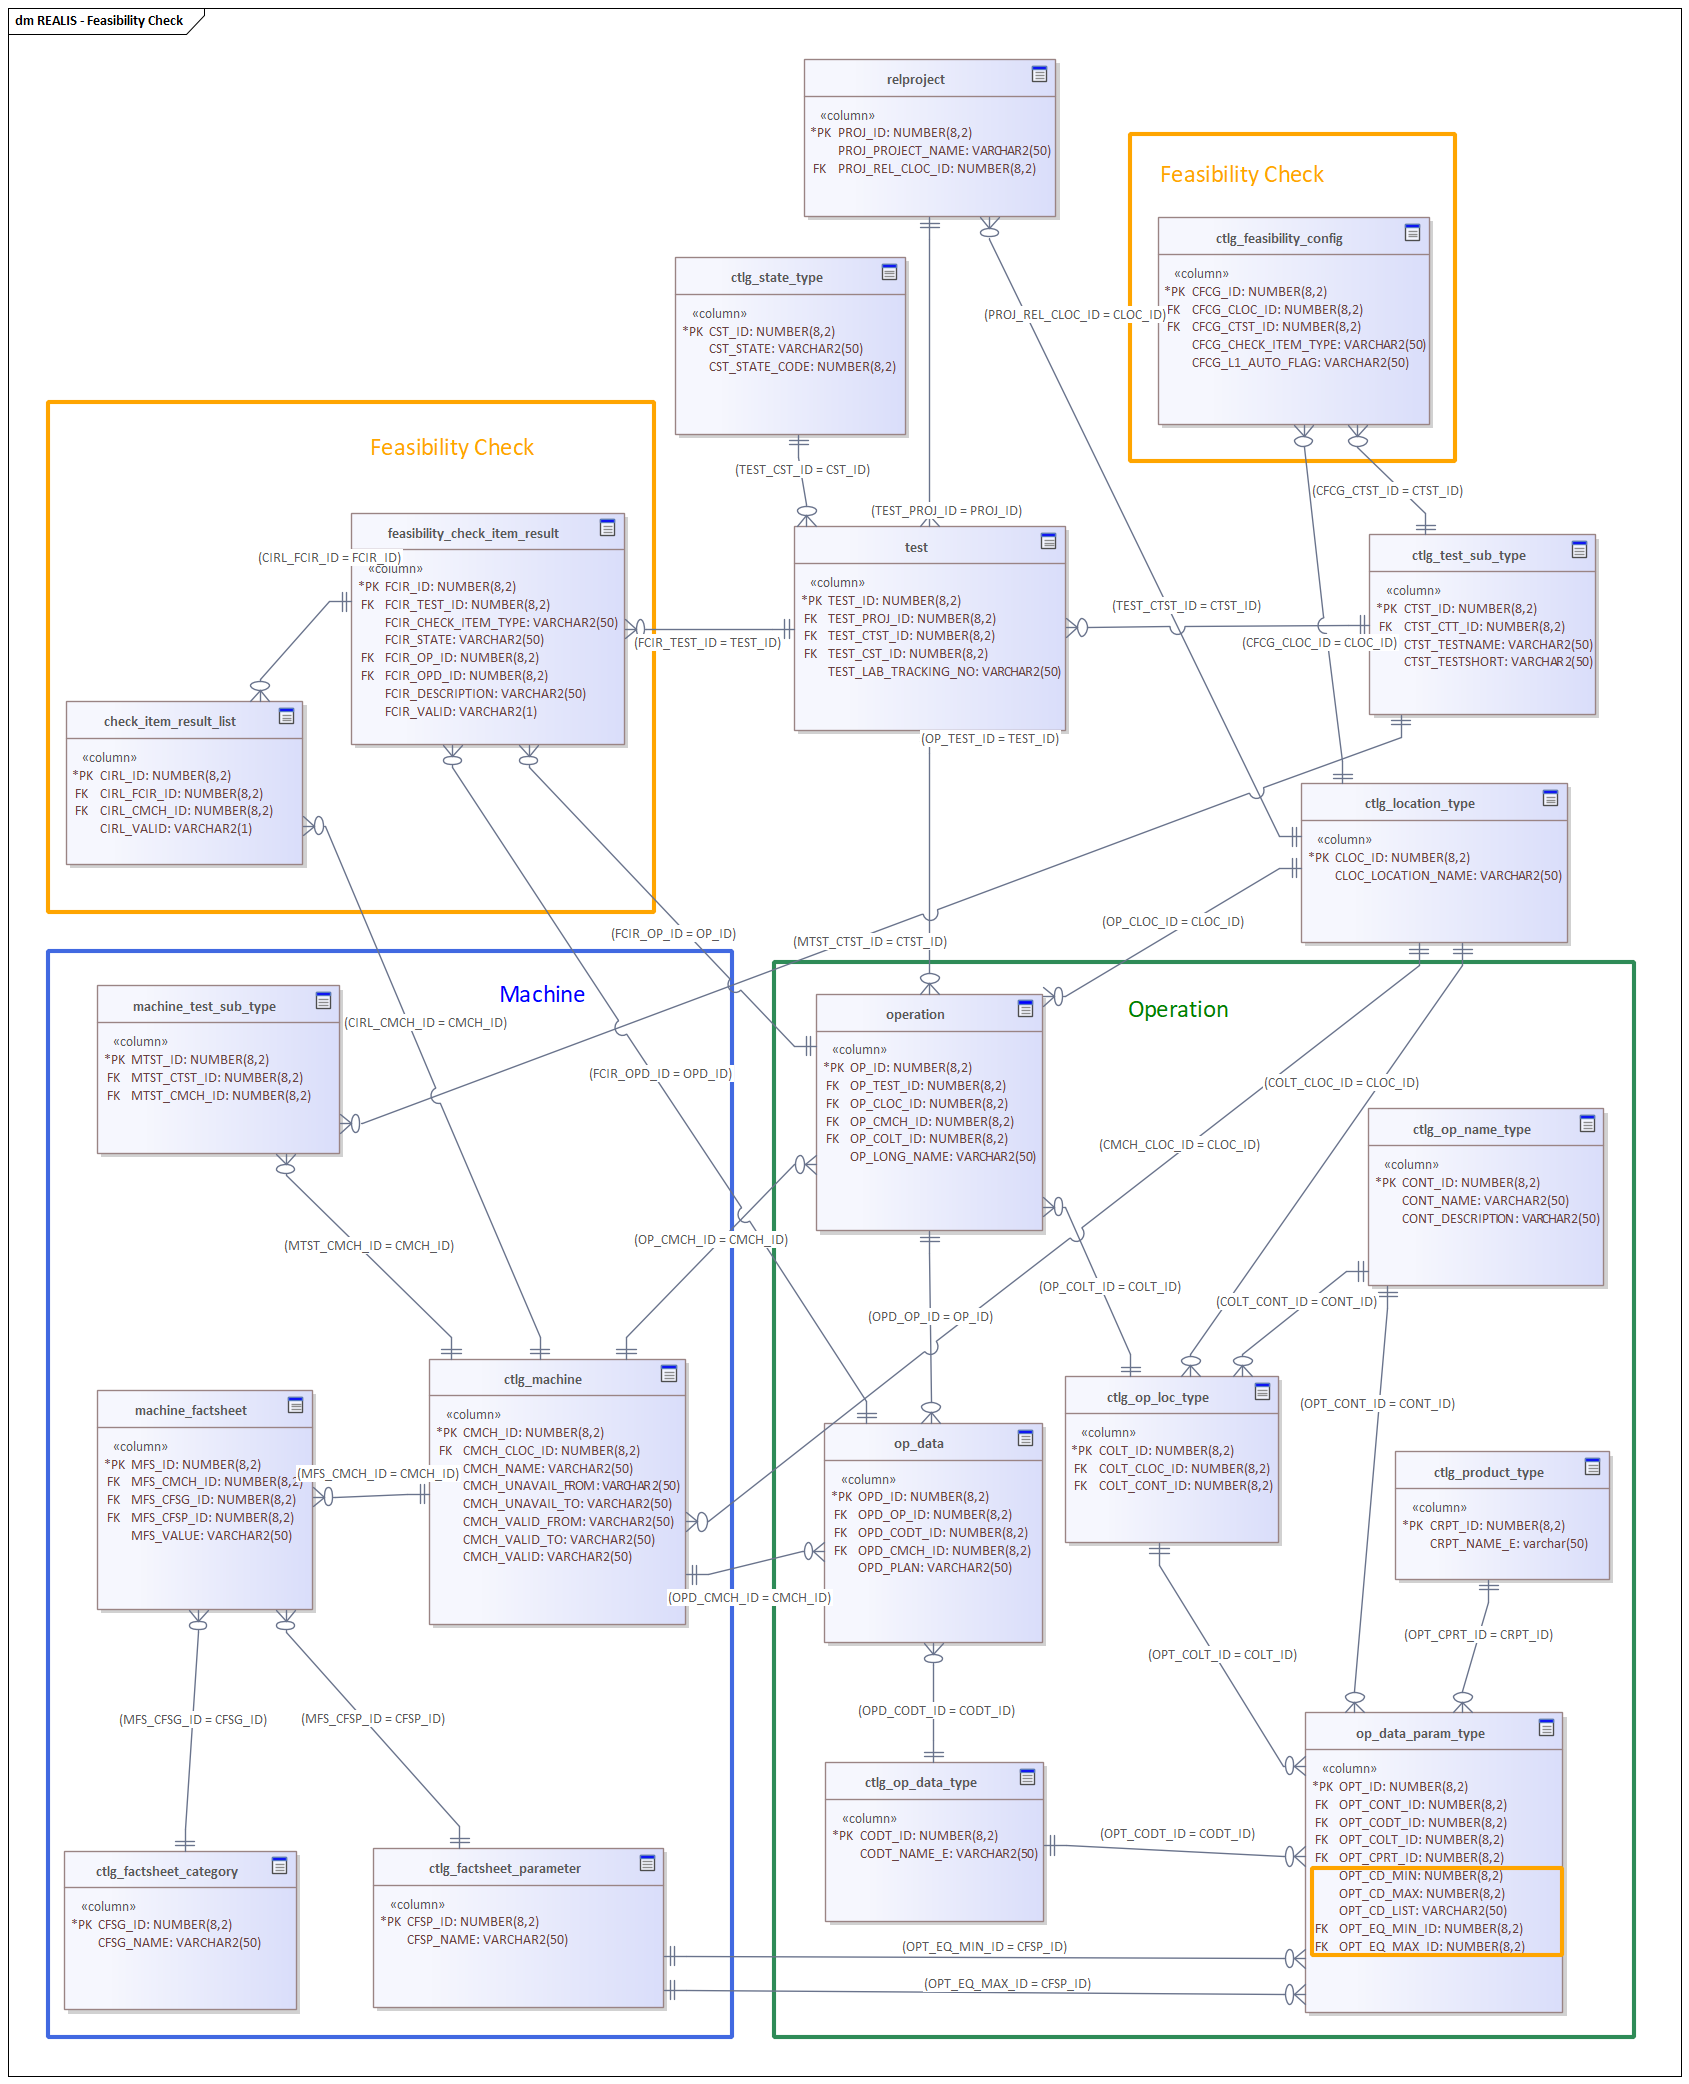
\includegraphics[width=0.98\paperwidth]{bilder/Datenbankdiagramm.png}}
    \caption{REALIS Datenbankdesign}
    \label{fig:realis-datenbankdesign}
\end{figure}

Die Tabelle \texttt{op\_name\_name\_type} bestimmt welche Arten von Operationen es gibt, und legt indirekt über die Tabelle \texttt{ctlg\_op\_loc\_type} fest, welche Operations-Typen auf welchen Standort verfügbar sind. Darüber hinaus definiert die 
\texttt{op\_data\_param\_type} Tabelle, welcher Parameter bei welcher Operation auf welchem Standort für welchen Produkttypen (\texttt{ctlg\_product\_type}) verfügbar ist. Hierbei sind der Standort und der Produkttyp aber nur optionale Einträge, um generische, standortübergreifende und/oder produktübergreifende Einträge zu realisieren.

Jeder (Stress-)Parameter einer Operation, der einen konkreten Wert definiert (\texttt{OPD\_PLAN}) muss von einer \textbf{Maschine} \texttt{ctlg\_machine} umgesetzt werden (können). Die eng mit der Maschine verknüpften Tabellen, befinden sich in der Abbildung \ref{fig:realis-datenbankdesign} im blau umrandeten Bereich. Eine Maschine ist verknüpft mit einem \textbf{Machinen-Test-Typen} (\texttt{machine\_test\_sub\_type}), der die Maschine einem Test-Typen zuordnet (\texttt{ctlg\_test\_sub\_type}). Außerdem besitzen Maschinen verschiedene \textbf{''Factsheets''} (\texttt{machine\_factsheet}) mit einem \textbf{Parameter} (\texttt{ctlg\_factsheet\_parameter}) und einem Wert (\texttt{MFS\_VALUE}). Dieser Wert korrespondiert mit der PlanValue (\texttt{OPD\_PLAN}) des Operations-Parameters. Hierbei gibt es aber (meist) für jeden Operations-Parameter-Typen zwei zugehörige Maschinen-Factsheet-Parameter(-Typen), die angeben, was jeweils das Minimum und das Maximum der Maschine, bei diesem Parameter ist.


\subsection{Datenbankerweiterung für Feasibility Check}

Für die Durchführung des Feasibility Checks muss die Datenbank erweitert werden. Dabei sollen die in Kapitel \ref{Subsec:ParameterdestechnischenFeasibilityChecks} beschriebenen Parameter und die zugrunde liegende Logik umgesetzt werden. Zusätzlich müssen die Anforderungen aus Kapitel \ref{Chap:Anforderungen} berücksichtigt werden.

Der Feasibility Check bewertet den Parameter-Wert einer (Stress-)Operation in zwei Dimensionen. Die Überprüfung der \textbf{Sinnhaftigkeit} \gls{ConditionCheck} und die Überprüfung der \textbf{Durchführbarkeit} \gls{EquipmentCheck}.
Dieser Parameter-Wert entspricht in der Datenbank REALIS dem Eintrag \textbf{\texttt{OPD\_PLAN}} in der Tabelle \texttt{op\_data}, die ihn definiert und den Parameter darstellt.

\textbf{\gls{ConditionCheck}} \\
Damit dieser Parameter-Wert auf Sinnhaftigkeit überprüft werden kann, werden in der generischen Tabelle \texttt{op\_data\_param\_type}, die Operationstyp, Parametertyp,  Standort und Produkttyp miteinander verknüpft, zwei neue Einträge hinzugefügt. Diese zwei Einträge beinhalten Werte, die den ''sinnvollen'' Bereich festlegen.

\setlength{\leftskip}{1em} 
\textbf{\texttt{OPT\_CD\_MIN}} - definiert die untere Grenze des zulässigen Wertebereichs

\textbf{\texttt{OPT\_CD\_MAX}} - legt die obere Grenze fest

\setlength{\leftskip}{0em} 

\textbf{\gls{EquipmentCheck}} \\
Für den \gls{EquipmentCheck} wird ebenfalls die Tabelle \texttt{opd\_data\_param\_type} um zwei Einträge ergänzt:

\setlength{\leftskip}{1em} 
\textbf{\texttt{OPT\_EQ\_MIN\_ID}} - Referenz auf den minimalen Maschinen-Parameter

\textbf{\texttt{OPT\_EQ\_MAX\_ID}} - Referenz auf den maximalen Maschinen-Parameter

\setlength{\leftskip}{0em} 

Diese Einträge dienen als Fremdschlüssel zu zwei Maschinen-Parametertypen (\texttt{ctlg\_factsheet\_parameter}), wobei einer der beiden dem ''minimalen'' Parameter und der andere dem ''maximalen'' Parameter entspricht. Die tatsächlichen Parameter-Werte stehen dann in der verknüpften \texttt{machine\_factsheet} Tabelle, in dem Feld \texttt{MFS\_VALUE}.

Jede Maschine, die einen bestimmten Operations-Parameter unterstützt, besitzt zwei zugehörige FactSheet-Parameter, die in der machine\_factsheet-Tabelle den minimalen und maximalen Wertebereich für diesen Parameter festlegen. Dadurch wird sichergestellt, dass alle relevanten Maschinen mit den entsprechenden Parametern verknüpft sind und dass für jede Maschine die jeweiligen Grenzen des umsetzbaren Wertebereichs definiert werden.


\textbf{Konfigurierbarkeit des automatisierten Feasibility Checks} \\
Bevor der automatisierte Feasibility Check vollständig ausgerollt wird, soll dieser umfassend getestet werden können. Dazu wird eine Konfigurationsmöglichkeit in der Datenbank geschaffen. Die Tabelle \textbf{\texttt{ctlg\_feasibility\_config}} ermöglicht die Festlegung, welche Tests bereits durch das neue System geprüft werden sollen und welche weiterhin einer manuellen Überprüfung unterliegen.

\setlength{\leftskip}{1em}

\textbf{Automatisierungsstatus} (\texttt{CFCG\_L1\_AUTO\_FLAG}) - legt fest, ob ein Test automatisiert oder manuell durchgeführt wird

\textbf{Standortabhängigkeit} (\texttt{CFCG\_CLOC\_ID}) - Berücksichtigung des jeweiligen (Labor-)Standorts

\textbf{Test-Typ} (\texttt{CFCG\_CTST\_ID}) - Differenzierung nach spezifischen Testarten

\textbf{Check-Typ} (\texttt{CFCG\_CHECK\_ITEM\_TYPE}) - definiert, ob es sich um einen \gls{ConditionCheck} oder einen \gls{EquipmentCheck} handelt

\setlength{\leftskip}{0em} 


\textbf{Speicherung der Feasibilitiy Check Ergebnisse} \\
Die Ergebnisse der durchgeführten Feasibility Checks werden in der Tabelle \textbf{\texttt{feasibility\_check\_item\_result}} gespeichert. Diese ist mit dem jeweiligen Test verknüpft und kann – sofern zutreffend – auch mit weiteren Ebenen wie der Operation oder einzelnen Parametern assoziiert werden. Diese Verknüpfungen sind jedoch optional, da in manchen Fällen bereits auf Testebene eine abschließende Bewertung möglich ist oder der Test keine spezifischen Operationen und Parameter umfasst.

Das Ergebnis eines Checks wird abhängig vom jeweiligen Check-Typ gespeichert. Zusätzlich enthält die Tabelle die folgenden Felder:

\setlength{\leftskip}{1em}

\texttt{FCIR\_STATE} – speichert den Status des Checks.

\texttt{FCIR\_DESCRIPTION} – dokumentiert die Begründung des Ergebnisses in Textform.

Gültigkeitskennzeichnung – eine zusätzliche "Flag" markiert, ob das Ergebnis aktuell gültig ist.

\setlength{\leftskip}{0em}

Da der Feasibility Check für einen Test mehrfach durchgeführt werden kann, bleiben vorherige Ergebnisse erhalten. Sobald jedoch ein neuer Check erfolgt, werden die vorherigen Ergebnisse als ungültig markiert.

Falls der \gls{EquipmentCheck} erfolgreich ist, müssen zusätzlich die Maschinen gespeichert werden, die für die geforderten Parameter geeignet sind. Diese werden in der Tabelle \textbf{\texttt{check\_item\_result\_list}} hinterlegt, die eine Verknüpfung zwischen den gefundenen Maschinen und dem jeweiligen Feasibility-Check-Ergebnis herstellt.

Außerdem werden zwei neue Stati in der Tabelle \texttt{ctlg\_state\_type} eingeführt. Zum einen ''FEASIBILITYREQUESTED'', dieser wird einem Test direkt nach dem Triggern des Feasibility Checks. Und einen zweiten: ''MANUALFEASIBILITY'' falls, der Test gescheitert ist. Ist der Test erfolgreich, wird er auf den bereits existierenden Status ''APPLY'' (bzw. ''FEASIBLE'') gesetzt. 



